\section{Diffusion}

For this exercise the new script ljanalyze.py was created.
It reads the data ot of a *.dat-file which is given by --ID like in ljsim.py.

\subsection{Implementation}

\subsubsection{Mean Squared Displacement (MSD)}

The MSD is defined by:
\begin{align}
\lk \D x^2\rk\lc \D t\rc
	&= \frac{1}{N}\sum_{k=1}^{N}\abs{\ovec{x}\lc k\D t\rc - \ovec{x}\lc\lc k-1\rc\D t\rc}^2
	\label{MSD}
\end{align}

Notice that $\D t$ is not the simulation timestep, but a duration for a sub-trajectory. 
Later it will be in $(0,T]$ where $T$ is the simulation time.

From the MSD we can derive the diffusion constant $D$ by fitting the following expression to the MSD.
\begin{align}
\lk \D x^2\rk 
	&= 2D_xd\D t
	\label{fit}
\end{align}

Where $d=3$ is the dimension of $\ovec{x}$.
The $x$ in $D_x$ means that it was derived from the position because later we derive it from the velocity $v$.\\

The function calc\_msd() performs equation \eqref{MSD}.
The while loop in line 61 goes over all possible $0 < k\D t < T$.
Because of the fact, that the simulation times (nearly) equal their index ndt is an integer.

\listfile{../src/ljanalyze.py}{src/ljanalyze.py}{54}{64}{MSD calculation}{calcmsd}

In the main loop (code block \ref{msdmain}) the calculation is done for all $\D t$ in steps of 1 until dtmax is reached. 
You can set dtmax by --dtmax; its default is $T$.

\listfile{../src/ljanalyze.py}{src/ljanalyze.py}{81}{88}{MSD main loop}{msdmain}
 
In the main loop also an error is detected by calc\_err().
It works like:
\begin{align}
\D \lk \D x^2\rk
	&=\sqrt{\frac{
		\sum_{k=1}^{N}\lb\abs{\ovec{x}\lc k\D t\rc - \ovec{x}\lc\lc k-1\rc\D t\rc}^2 
		- \lk \D x^2\rk\rb ^2}{N\cdot\lc N-1\rc}}
\end{align}

You can see the code in code block \ref{calcerr}.
 
\listfile{../src/ljanalyze.py}{src/ljanalyze.py}{66}{79}{MSD error}{calcerr}

As you can see the error is set to zero if $N=1$ in line 78-79 in order to provide division by zero.
In this area no representative error can be estimated any more.\\

The fit is done with a simple order 1 numpy.polyfit().
Furthermore you can pass the regression limits via --linreg <min> <max>.

\listfile{../src/ljanalyze.py}{src/ljanalyze.py}{92}{94}{MSD Fit}{msdfit}

\subsubsection{Velocity autocorrelation Function (VACF)}

Another way to find the diffusion constant (now $D_v$) is via the VACF.
It is defined by:
\begin{align}
\text{VACF}(t)
	&=\lk \ovec{v}(t) \cdot \ovec{v}(0) \rk 
	\label{vacf}\\
	&\approx \text{normed}\lb\text{ifft}\lc \overline{\text{fft}(\ovec{v})} \cdot \text{fft}(\ovec{v})\rc\rb\label{fft}
\end{align}

It can be derived from a discrete velocity vector $\ovec{v}$ via Fast Fourier Transformation fft (inverse: ifft).
Normed means that VACF$(0) = 1$.

This Autocorrelation is implemented in code block \ref{autocor}.
The calculation of fft is split up into the 3 dimensions. 
In line 118 they are added.
Furthermore the while statement in 117 is not necessary for the task but allows the usage for other shapes (n,m,...) or 1D-arrays.

\listfile{../src/ljanalyze.py}{src/ljanalyze.py}{110}{119}{Autocorrelation function}{autocor}

$D_v$ now can be derived by integrating over the VACF (Green-Kubo relation).
This is done in the script with numpy.trapz.

\subsection{Analyze}

\begin{figure}[ht]
	\centering
	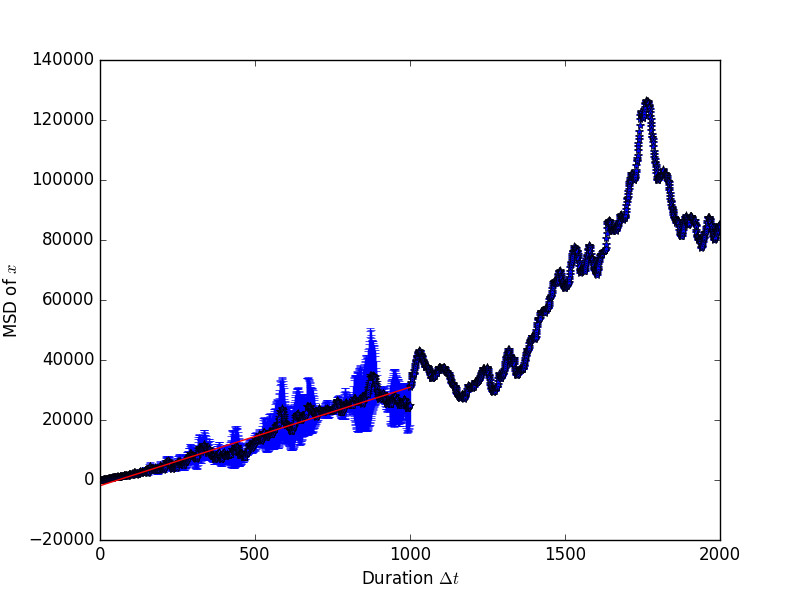
\includegraphics[width=0.5\textwidth]{../dat/langevin_T1d0_gamma0d3_MSD.png}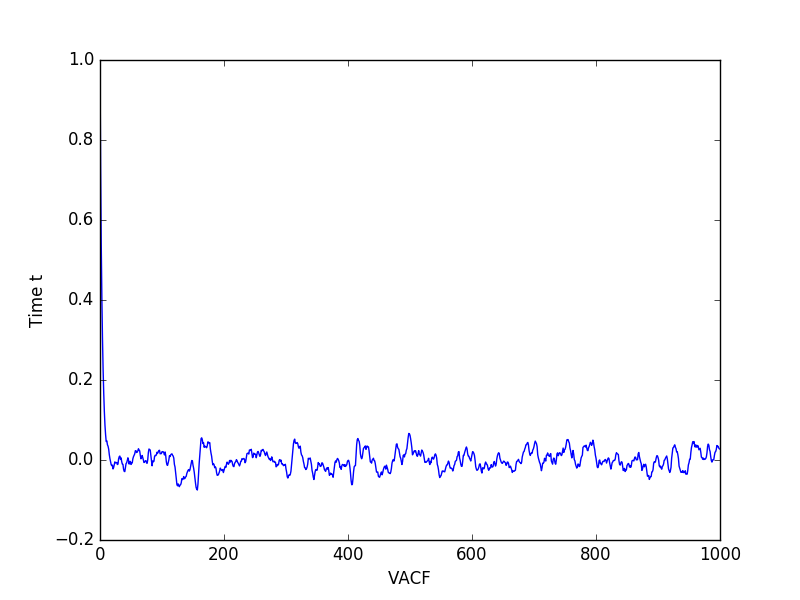
\includegraphics[width=0.5\textwidth]{../dat/langevin_T1d0_gamma0d3_VACF.png}
	\caption{
		Plot of the MSD (left) and the VACF (right) for a desired temperature of $T_\text{des}=1.0$ for a simulation with the Langevin thermostat and $\gamma =0.3$.
	}
	\label{langevin3}
\end{figure}


\begin{figure}[ht]
	\centering
	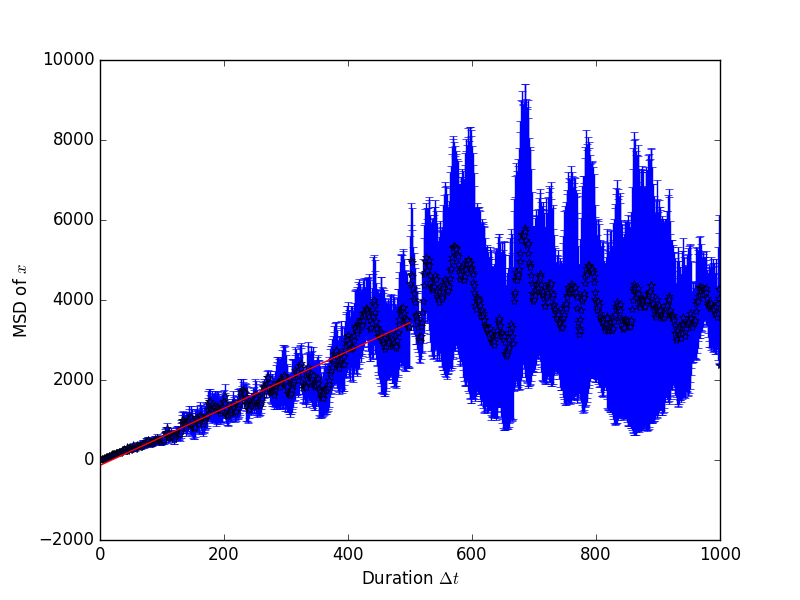
\includegraphics[width=0.5\textwidth]{../dat/langevin_T1d0_gamma0d8_MSD.png}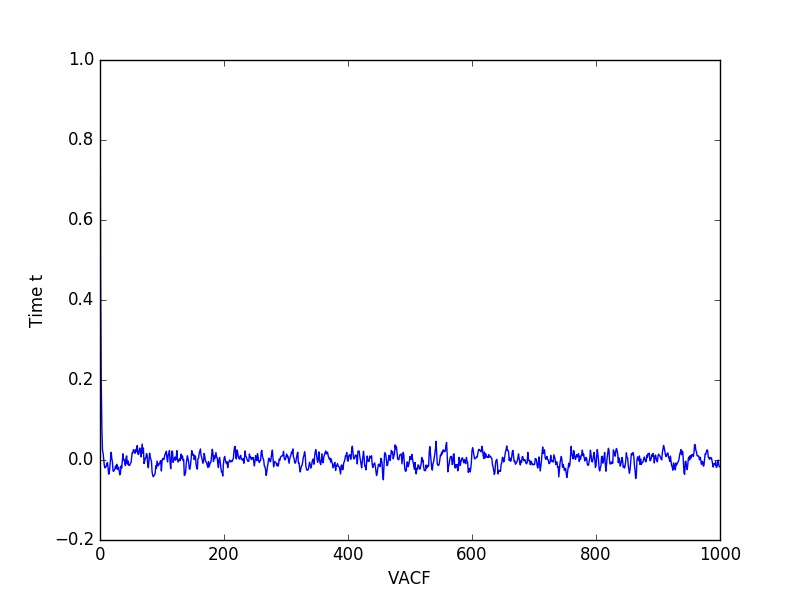
\includegraphics[width=0.5\textwidth]{../dat/langevin_T1d0_gamma0d8_VACF.png}
	\caption{
		Plot of the MSD (left) and the VACF (right) for a desired temperature of $T_\text{des}=1.0$ for a simulation with the Langevin thermostat and $\gamma =0.8$.
	}
	\label{langevin8}
\end{figure}


\begin{figure}[ht]
	\centering
	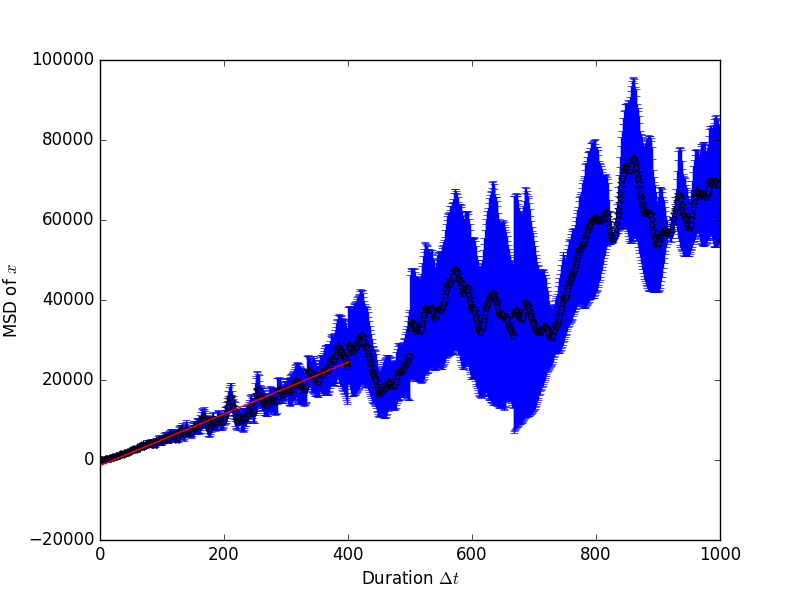
\includegraphics[width=0.5\textwidth]{../dat/langevin_T1d0_gamma0d1_MSD.png}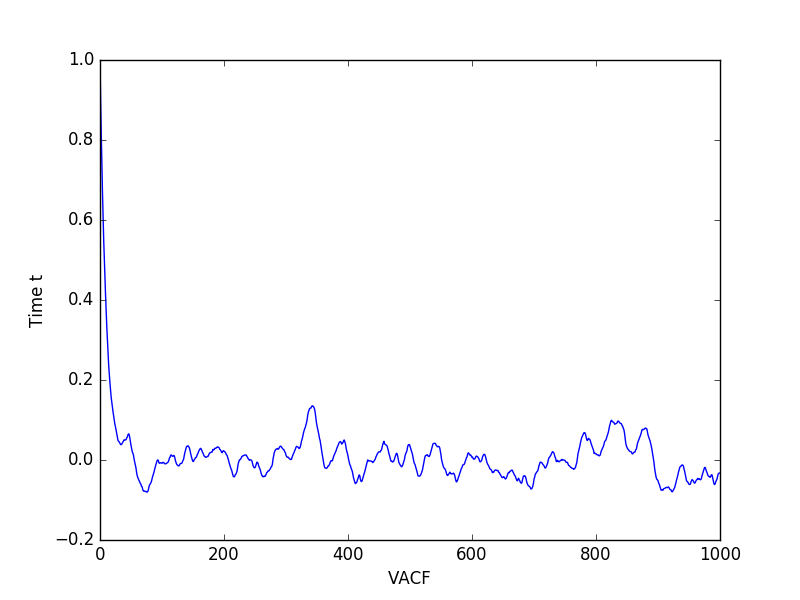
\includegraphics[width=0.5\textwidth]{../dat/langevin_T1d0_gamma0d1_VACF.png}
	\caption{
		Plot of the MSD (left) and the VACF (right) for a desired temperature of $T_\text{des}=1.0$ for a simulation with the Langevin thermostat and $\gamma =0.1$.
	}
	\label{langevin1}
\end{figure}

\begin{figure}[ht]
	\centering
	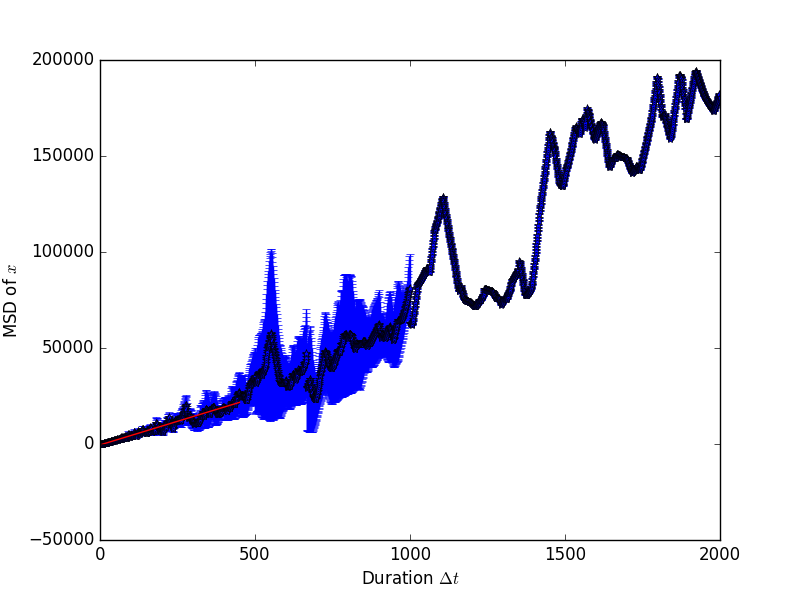
\includegraphics[width=0.5\textwidth]{../dat/andersen_T1d0_nu0d1_MSD.png}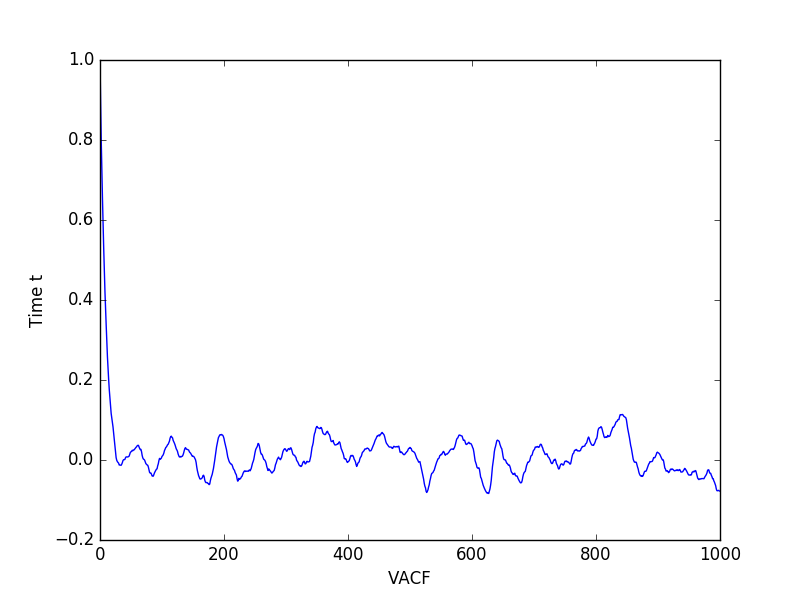
\includegraphics[width=0.5\textwidth]{../dat/andersen_T1d0_nu0d1_VACF.png}
	\caption{
		Plot of the MSD (left) and the VACF (right) for a desired temperature of $T_\text{des}=1.0$ for a simulation with the Andersen thermostat and $\nu =0.1$.
	}
	\label{andersennana0}
\end{figure}

\begin{figure}[ht]
	\centering
	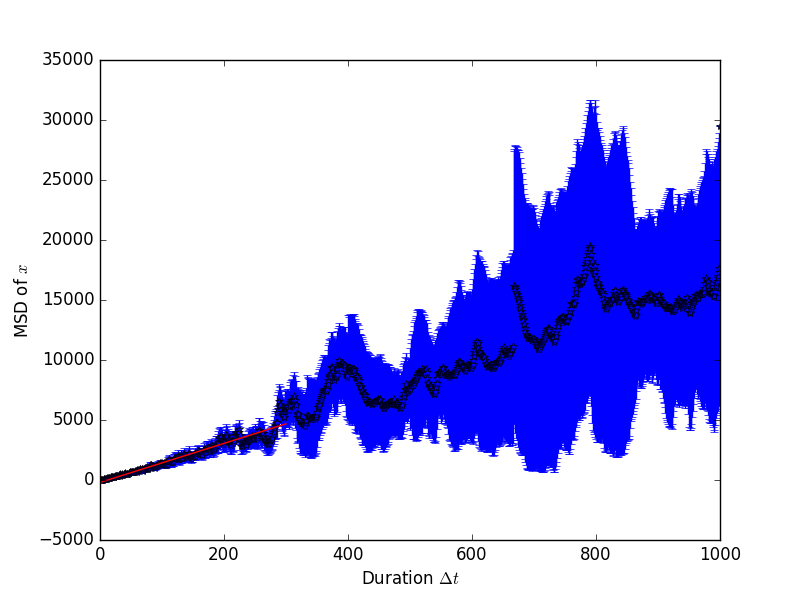
\includegraphics[width=0.5\textwidth]{../dat/andersen_T1d0_nu0d5_MSD.png}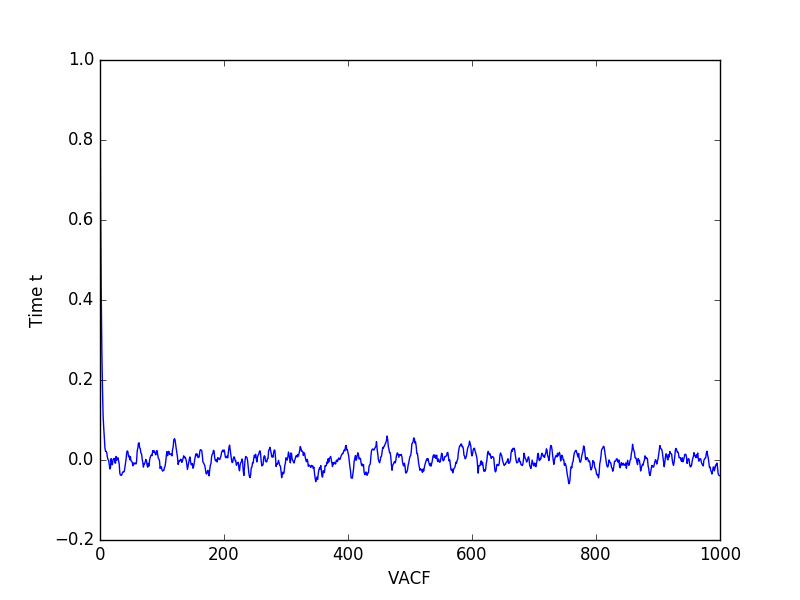
\includegraphics[width=0.5\textwidth]{../dat/andersen_T1d0_nu0d5_VACF.png}
	\caption{
		Plot of the MSD (left) and the VACF (right) for a desired temperature of $T_\text{des}=1.0$ for a simulation with the Andersen thermostat and $\nu =0.5$.
	}
	\label{andersennana5}
\end{figure}

\begin{figure}[ht]
	\centering
	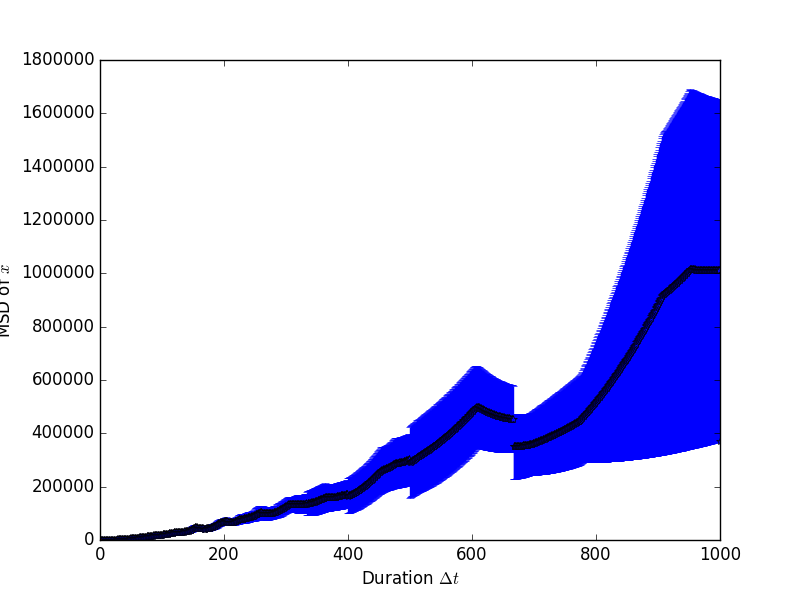
\includegraphics[width=0.5\textwidth]{../dat/andersen_T1d0_nu0d01_MSD.png}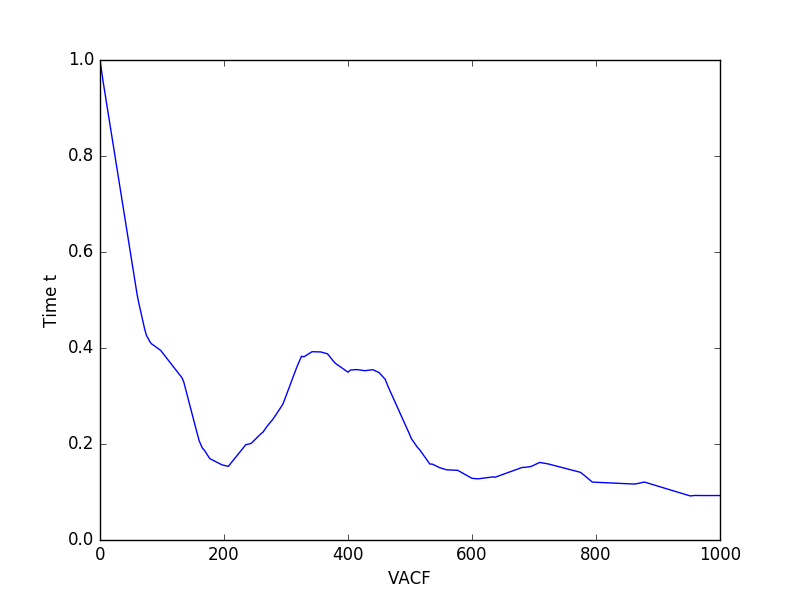
\includegraphics[width=0.5\textwidth]{../dat/andersen_T1d0_nu0d01_VACF.png}
	\caption{
		Plot of the MSD (left) and the VACF (right) for a desired temperature of $T_\text{des}=1.0$ for a simulation with the Andersen thermostat and $\nu =0.01$.
	}
	\label{andersennana01}
\end{figure}

\begin{figure}[ht]
	\centering
	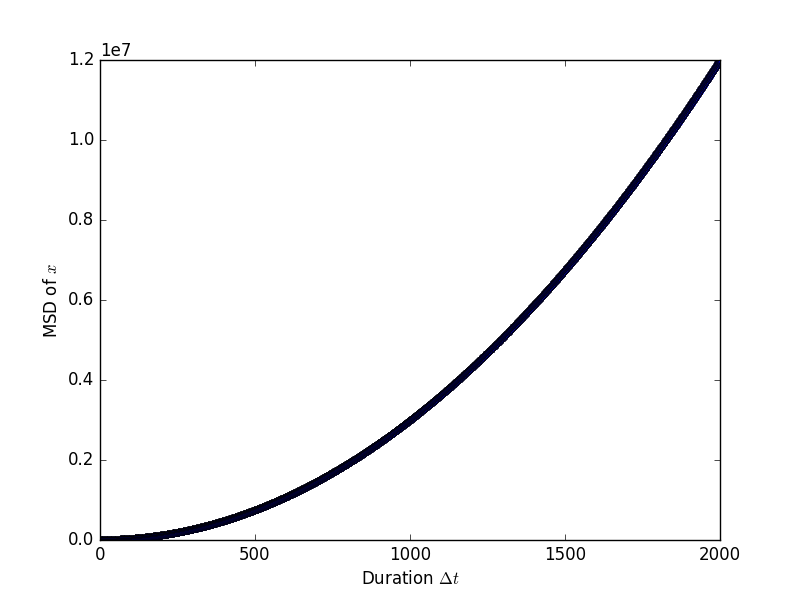
\includegraphics[width=0.5\textwidth]{../dat/berendsen_T1d0_tau3d0_MSD.png}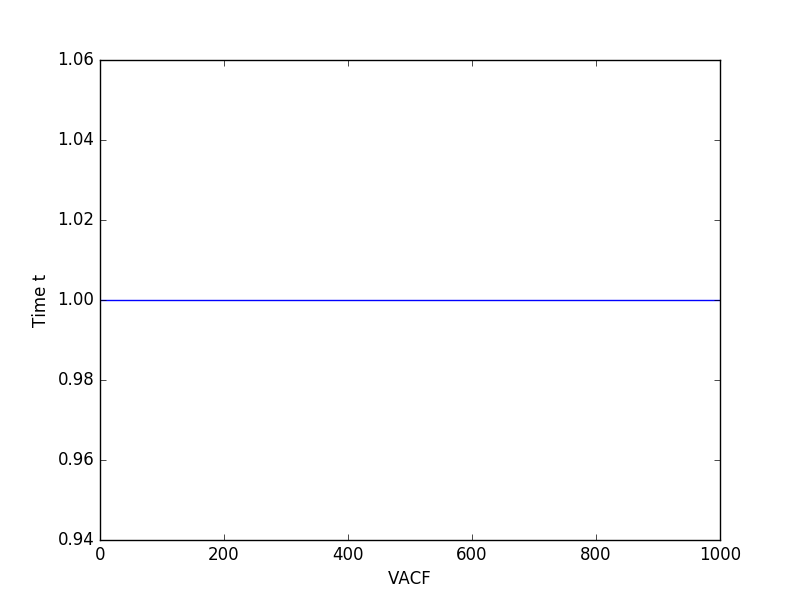
\includegraphics[width=0.5\textwidth]{../dat/berendsen_T1d0_tau3d0_VACF.png}
	\caption{
		Plot of the MSD (left) and the VACF (right) for a desired temperature of $T_\text{des}=1.0$ for a simulation with the Berendsen thermostat and $\tau_T =3.0$.
	}
	\label{berendsenana}
\end{figure}

Now we can analyze the simulation data.
Therefor some new data with different coefficients was created.
The plotted MSD and VACF is shown in the figures \ref{langevin3} until \ref{berendsenana}.\\

As you can see the MSD is only linear at the beginning. 
For higher $\D t$ the MSD fluctuates heavily because of the lesser number of values for the calculation.
As you can see for example in picture \ref{langevin3} the linear regression is only done in the area in which the red line is drawn.\\

By taking a look at figure \ref{berendsenana} you can see that there is no linear behaviour at all, but a quadratic behavior.
This is because the velocity does not change at all and therefor the distance $\D x$ grows linear in $t$ and the MSD therefor quadratic.\\

Figure \ref{andersennana01} shows that for tiny $\nu =0.01$ the behavior of the MSD also loose its linear beginning. 
There are not many collisions any more and the velocity is changed not often.
As consequence the curve is build up from quadratic like sub-curves.\\

In order to get an better overview the values of the diffusion constant are written to a tabular:

\begin{center}
	\begin{tabular}{l|sssss}
		Thermostat
		&\multicolumn{3}{c}{Langevin}
		&\multicolumn{2}{c}{Andersen}
		\\\hline
		$\gamma / \nu$
		&0.1
		&0.3
		&0.8
		&0.1
		&0.5
		\\
		$D_x$
		&10.76
		&2.59
		&1.19
		&9.15
		&2.71
		\\
		$D_v$
		&10.06
		&2.64
		&1.11
		&15.90
		&2.68
	\end{tabular}\\
\end{center}

This values show that it the values $D_x$ and $D_v$ are very similar for the l=Langevin thermostat.
But this may also depend on "good" choices of the regression interval.\\

As you can see the diffusion decreases with growing friction constant $\gamma$ and also with an growing collision probability $\nu$.
This is due to the fact that the more random walk influences the simulation the less the position $\abs{\ovec{x}}$ will change over time (in the stochastic average).



